\chapter{Methods}\label{chap:methods}

% Describe the method/software/tool/algorithm you have developed here

In the preceding chapters, all the necessary background knowledge to understand the methods have been introduced. In this chapter, we will present an overview of the challenges, the methods, and the tools we have developed for this thesis. We will first describe the dataset we have used. Then, we will describe the programs developed for this thesis. Finally, we will describe how we have packaged and deployed our programs with Nix.


% * collaboration between clément and I
% * timeline of the project
% * the architecture for computations, personal machine, remote server
% * packaging and deployment with Nix

\section{OpenSSH memory dumps dataset}\label{sec:background:kex:dataset}

    SmartKex has contributed to the research community by generating a comprehensive annotated dataset of OpenSSH heap memory dumps \cite{SmartKex22}. The dataset is publicly available on Zenodo \footnote{\url{https://zenodo.org/record/6537904}}. 

    \begin{minipage}{\dimexpr\linewidth-20pt}
        The dataset is organized into two top-level directories: $Training$ and $Validation$ with an additional $Performance\_Test$. The first two main directories are further divided based on the SSH scenario, such as immediate exit, port-forward, secure copy, and shared connection. Each of these subdirectories is then categorized by the software version that generated the memory dump. Within these, the heaps are organized based on their key lengths, providing a multi-layered structure that aids in specific research queries.

        \begin{figure}[H]
            \centering
            \caption{Illustration of the Dataset Directory Structure}
            \label{fig:dataset_structure}
            \begin{minipage}{0.6\textwidth}
            \dirtree{%
            .1 /.
            .2 Performance\_Test.
            .3 V\_7\_1\_P1.
            .4 16.
            .4 24.
            .4 32.
            .3 ....
            .2 Training.
            .3 basic.
            .4 V\_6\_0\_P1.
            .5 16.
            .5 24.
            .5 32.
            .4 ....
            .3 ....
            .2 Validation.
            .3 basic.
            .4 V\_6\_0\_P1.
            .5 16.
            .5 24.
            .5 32.
            .4 ....
            .3 ....
            }
        \end{minipage}
        \end{figure}
    \end{minipage}

    Two primary file formats are used to store the data: JSON and RAW. The JSON files contain meta-information like the encryption method, virtual memory address of the key, and the key's value in hexadecimal representation. The RAW files, on the other hand, contain the actual heap dump of the OpenSSH process.

    \begin{minipage}{\dimexpr\linewidth-20pt}
        Here is an example of content of a RAW memory dump file, displayed using \textit{vim} and \textit{xdd} commands:

        \begin{lstlisting}[style=hexdump, caption={16 bytes per line visualization of a Hex Dump from \textit{Training/basic/V\_7\_8\_P1/16/5070-1643978841-heap.raw}}]
            00000000: 0000 0000 0000 0000 5102 0000 0000 0000  ........Q.......
            00000010: 0607 0707 0707 0303 0200 0006 0401 0206  ................
            00000020: 0200 0001 0100 0107 0604 0100 0000 0203  ................
            00000030: 0103 0101 0000 0000 0000 0000 0000 0002  ................
            00000040: 0001 0000 0000 0000 0000 0100 0000 0001  ................
            00000050: 8022 1a3a 3456 0000 007f 1a3a 3456 0000  .".:4V.....:4V..
            00000060: f040 1a3a 3456 0000 9032 1a3a 3456 0000  .@.:4V...2.:4V..
            00000070: 608b 1a3a 3456 0000 9047 1a3a 3456 0000  `..:4V...G.:4V..
        \end{lstlisting}
    \end{minipage}

    The original file contains the raw byte content of the heap dump of a specific version of OpenSSH. It is a binary file, which means that it is not human-readable. However, it can be converted to a human-readable format using the \textit{xxd} command. The first column to the left represents the offset in hexadecimal. The last column represents the actual content of the bytes, in ASCII format. The columns in between represent the content of the bytes in hexadecimal format.

    Since hexadecimal is a base-16 number system, each byte is represented by two hexadecimal digits. The ASCII representation of the bytes is displayed on the right, and is only used for reference, as it is not always possible to convert the bytes to ASCII. For instance, the bytes at offset 0x10 are not printable characters, and thus cannot be converted to ASCII. Each line represents 16 bytes, and the offset is incremented by 16 for each line.

    For the purpose of this thesis, it will be more interesting to visualize the content of the heap dump as 8 bytes lines. This can be achieved by using the \textit{xxd} command with the \textit{-c} option, as shown in the following example:

    \begin{minipage}{\dimexpr\linewidth-20pt}
        The same example as before, a memory dump file, displayed using \textit{vim} and \textit{xdd -c 8} commands:

        \begin{lstlisting}[style=hexdump, caption={8 bytes per line visualization of a Hex Dump from \textit{Training/basic/V\_7\_8\_P1/16/5070-1643978841-heap.raw}}, label={lst:hexdump-8bytes}]
            00000000: 0000 0000 0000 0000  ........
            00000008: 5102 0000 0000 0000  Q.......
            00000010: 0607 0707 0707 0303  ........
            00000018: 0200 0006 0401 0206  ........
            00000020: 0200 0001 0100 0107  ........
            00000028: 0604 0100 0000 0203  ........
            00000030: 0103 0101 0000 0000  ........
            00000038: 0000 0000 0000 0002  ........
            00000040: 0001 0000 0000 0000  ........
            00000048: 0000 0100 0000 0001  ........
            00000050: 8022 1a3a 3456 0000  .".:4V..
            00000058: 007f 1a3a 3456 0000  ...:4V..
            00000060: f040 1a3a 3456 0000  .@.:4V..
            00000068: 9032 1a3a 3456 0000  .2.:4V..
            00000070: 608b 1a3a 3456 0000  `..:4V..
            00000078: 9047 1a3a 3456 0000  .G.:4V..
        \end{lstlisting}
    \end{minipage}

    This example shows the exact content of the preceding one. 

    To this RAW file is associated a JSON file, which contains its annotations.  

    \begin{minipage}{\dimexpr\linewidth-20pt}
         Here is a example of content of a JSON annotation file that comes with the previous RAW file:

        %\begin{lstlisting}[language=json, , ]
        \begin{lstlisting}[style=json, caption={Complete JSON example, from \textit{Training/basic/V\_7\_8\_P1/16/5070-1643978841.json}}, label={lst:json-annotation-ex-1}]
            {
                "SSH_PID": "5070",
                "SSH_STRUCT_ADDR": "56343a1a4800",
                "session_state_OFFSET": "0",
                "SESSION_STATE_ADDR": "56343a1a8d30",
                "newkeys_OFFSET": "344",
                "NEWKEYS_1_ADDR": "56343a1aaa40",
                "NEWKEYS_2_ADDR": "56343a1aab40",
                "enc_KEY_OFFSET": "0",
                "mac_KEY_OFFSET": "48",
                "name_ENCRYPTION_KEY_OFFSET": "0",
                "ENCRYPTION_KEY_1_NAME_ADDR": "56343a1a9db0",
                "ENCRYPTION_KEY_1_NAME": "aes128-gcm@openssh.com",
                "ENCRYPTION_KEY_2_NAME_ADDR": "56343a1a3fb0",
                "ENCRYPTION_KEY_2_NAME": "aes128-gcm@openssh.com",
                "key_ENCRYPTION_KEY_OFFSET": "32",
                "key_len_ENCRYPTION_KEY_OFFSET": "20",
                "iv_ENCRYPTION_KEY_OFFSET": "40",
                "iv_len_ENCRYPTION_KEY_OFFSET": "24",
                "KEY_A_ADDR": "56343a1a3170",
                "KEY_A_LEN": "12",
                "KEY_A_REAL_LEN": "12",
                "KEY_A": "feb5fd4ef0759b034d69b858",
                "KEY_B_ADDR": "56343a1a33e0",
                "KEY_B_LEN": "12",
                "KEY_B_REAL_LEN": "12",
                "KEY_B": "f50b988297fa19709445c4ee",
                "KEY_C_ADDR": "56343a1aa1b0",
                "KEY_C_LEN": "16",
                "KEY_C_REAL_LEN": "16",
                "KEY_C": "f5b53280e944db0fe196668d877cd4c0",
                "KEY_D_ADDR": "56343a1a4010",
                "KEY_D_LEN": "16",
                "KEY_D_REAL_LEN": "16",
                "KEY_D": "ac4f18a963d9e72c857497b7dc9d088d",
                "KEY_E_ADDR": "56343a1a7d90",
                "KEY_E_LEN": "0",
                "KEY_E_REAL_LEN": "0",
                "KEY_E": "",
                "KEY_F_ADDR": "56343a1a2f60",
                "KEY_F_LEN": "0",
                "KEY_F_REAL_LEN": "0",
                "KEY_F": "",
                "HEAP_START": "56343a198000"
            }
        \end{lstlisting}
    \end{minipage}

    Those annotation files contain the meta-information about the heap dump, such as the encryption method, virtual memory address of the key, and the key's value in hexadecimal representation. Those annotations are invaluable for the development of machine learning models for key extraction. 

    The dataset is not just limited to SSH key extraction; it also serves as a resource for identifying essential data structures that hold sensitive information. This makes it a versatile tool for various research applications, including but not limited to machine learning models for key extraction and malware detection. 

    \subsection{Assumptions}
    Before we dive in, let's make some assumptions about the dataset. We will use these assumptions to guide our exploration of the heap dump file. 

    \begin{itemize}
        \item \textbf{Heap dump file size:} We will assume that the heap dump file size is a multiple of 8 bytes. This is because the heap dump file is a memory dump, and memory is allocated in chunjs that are multiples of 8 bytes. This means that we can expect the heap dump file to be composed of a sequence of 8 bytes blocks. If this assumption is not met, we will assume that padding the last block with 0s will not change the results of our exploration.
        \item \textbf{Malloc header chaining:} We will assume that all the heap dump files have been generated using the same \lstinline[language=c]|malloc| implementation. It means that we can expect to find the same patterns in all the heap dump files. Especially, we expect all the heap dump files to start by zero or more blocks of 8 bytes of 0s, followed by the first malloc header. We can then follow the malloc header chaining to explore the heap dump file allocated memory chunks.
        \item \textbf{Dataset key annotation format:} We will assume that the JSON annotation files have been generated using the same program. This means that we can expect the same format for all the JSON annotation files. This is important, as we will use the JSON annotation files to get the key addresses for annotating memory graphs used for the embedding step. If the format is not the same, we will assume that the JSON annotation file is corrupted, and we will skip it.
    \end{itemize}

    In the scripts and programmed that have been developped for the following thesis, we have implemented a number of checks and tests to ensure that these assumptions are met. If not, the programs will raise an error, log the problem and generally skip the data. This behavior is implemented to ensure that the programs are robust to unexpected data, and to ensure that the results are reliable. These assumptions, and related problems will be discussed and measured at several locations in the following sections.

    \subsection{Estimating the dataset balancing for key prediction}
    First, let's quickly estimate what the dataset is composed about. This will later be used to estimate the balancing of data for our key prediction goal. Some quick linux commands can be used to get a general overview of the dataset.
    
    A first command can quickly give us an idea of the number of files in the dataset:
    \begin{lstlisting}[caption={Count all dataset files}, label=methods:code:count_all_dataset_files, language=bash]
        find /path/to/dataset -type f | wc -l
    \end{lstlisting}

    Another command can be used to get the total size of the dataset:
    \begin{lstlisting}[caption={Get the total size of the dataset}, label=methods:code:get_total_size_dataset, language=bash]
        du -sb /path/to/dataset
    \end{lstlisting}

    The first command indicates that the dataset contains $ 208749 $ files, which represents, according to second one, a total of $ 18203592048 $ bytes, or around 18 Gigabytes.

    We could just divide the number of files by the size of the dataset to get an average size of the files. However, this would not be accurate, as we are only interested in the size of the RAW files. Since JSON files are much smaller than RAW files, they would skew the average size of the files. Since we are only considering RAW files, we will use improved commands in order to determine the size of the RAW file only.

    The following command can be used to get a better understanding of the dataset, concerning the number of RAW files and their size:

    \begin{lstlisting}[caption={Find the number of RAW files in the dataset}, language=bash]
        find /path/to/dataset -type f -name "*.RAW" | wc -l
    \end{lstlisting}

    And the next one can be used to get the number of bytes of RAW files in the dataset:

    \begin{lstlisting}[caption={Find the number of bytes of RAW files in the dataset}, language=bash]
        find /path/to/dataset -type f -name "*.raw" -exec du -b {} + \
            | awk '{s+=$1} END {print s}'
    \end{lstlisting}

    Where:
    \begin{itemize}
        \item \lstinline[language=bash]!find phdtrack_data/ -type f -name "*.raw"! finds all the files in the dataset that have the extension \lstinline[language=bash]!.raw!.
        \item \lstinline[language=bash]!-exec du -b {} + | awk '{s+=$1} END {print s}'! executes the command \lstinline[language=bash]!du -b! on each file found by the previous command, and sums the size of each file.
    \end{itemize}

    Theses commands indicate that the dataset contains $ 103595 $ RAW files, which represents a total of $ 18067001344 $ bytes, or around 18 Gigabytes. This shows that the vast majority of the data is contained in RAW files, with JSON files representing less than a percent of the dataset in term of byte size. As such, the average size for every RAW file is around 170 Kilobytes. 

    Now, considering that a given heap dump file is expecting to have only 6 keys (see \autoref{sec:background:ssh:ssh_keys}), with keys maximal possible size being of 64 bytes, we can estimate that we have at maximum $ 39780480 $ or around 40 Megabytes of positively labeled samples. This, considering the total useful size of around 18 Gigabytes, means that our dataset is very imbalanced, with an expected upper-bounded ratio of $ 0.0022\% $ of positively labeled samples or around $ 2:1000 $.

    Considering that, a frontal \acrshort{ml} binary classification approach will not work. This is why the present report will discuss feature engineering and graph-based memory representation. The idea is to embed more information to our keys so as to be able to fight effectively the imbalanceness of the raw data.

    \subsection{Dataset validation}
    The dataset is mearly a collection of heap dump RAW files for different use cases and versions of OpenSSH. Each heap dump file goes along a JSON annotation file that has been generated by the creators of the dataset to provide additional information about the heap dump, and especially encryption keys.
    
    However, it is worth noting that the dataset is not perfect, as some of the annotations are sometimes missing. This is probably due to the fact that the annotations were generated automatically, and some of the keys are missing. For instance, in \textit{Training/basic/V\_7\_8\_P1/16/}, literally the first file of the dataset contains an incomplete annotation file, as some of the keys are missing. This is a limitation of the dataset that should be kept in mind when using it for research purposes.

    \begin{minipage}{\dimexpr\linewidth-20pt}
        Here is an example of content of a JSON annotation file with missing keys, and with missing annotations (like address or lenght) for the keys that are present:

        \begin{lstlisting}[style=json, caption={Missing keys in JSON annotation file \textit{Training/basic/V\_6\_0\_P1/16/24375-1644243522.json}}]
            {
                "ENCRYPTION_KEY_NAME": "aes128-ctr",
                "ENCRYPTION_KEY_LENGTH": "16",
                "KEY_C": "689e549a80ce4be95d8b742e36a229bf",
                "KEY_D": "76788e66a56d2b61eec294df37422fcb",
                "HEAP_START": "5589d41e0000"
            }
        \end{lstlisting}
    \end{minipage}

    \subsubsection{Automatic annotation validation}
    So as to determine really how much of the dataset can be really for machine learned, we have developped a script that checks the validity of thoses annotations. This script called \texttt{check\_annotations.py}, is used to verify the quality, completeness, consistency and coherence of the annotations.

    Files are regroup under the following categories:

    \begin{itemize}
        \item \textbf{Correct and Complete Files:} Files that have no missing keys, and that have all the keys with correct values.
        \item \textbf{Broken Files:} Files that are not valid JSON files, and cannot be loaded as such.
        \item \textbf{Incorrect Files:} Files that have contradictory information in their annotation file.
        \item \textbf{Missing key Files:} Files that have missing keys in their annotation file. A typical example is a JSON file with \lstinline[style=json]!"KEY_E": ""!. This means that the key E is missing, and that the key E address is not present in the annotation file, which is a problem for the machine learning since it means that we cannot label correctly the key E.
        \item \textbf{Incomplete key Files:} Files that have incomplete keys in their annotation file. A typical example is a JSON file with \lstinline[style=json]!"KEY_E": "689e549a80ce4be95d8b742e36a229bf"!. This means that the key E is present, but that the key E address is not present in the annotation file, which is a problem for the machine learning since it means that we cannot label correctly the key E.
    \end{itemize}

    The script is used to validate each JSON file using the following process:

    \begin{algorithm}[H]
        \caption{Json Annotation Validation}
        \begin{algorithmic}[1]
        \Procedure{ValidateJson}{$\text{json\_data}$}
            \State \textbf{Initialize} errors = Dictionnary\{\} \Comment{Serve as collection for counted errors}
            \State \textbf{Initialize} mandatory\_json\_keys = ['HEAP\_START', 'SSH\_STRUCT\_ADDR', 'SESSION\_STATE\_ADDR']
            \State \textbf{Initialize} key\_names = \{\}
            \State \textbf{Initialize} incorrect\_keys, missing\_keys, incomplete\_keys = 0
            
            \For{mandatory\_json\_key \textbf{in} mandatory\_json\_keys} \Comment{Check if some expected json keys are missing}
                \If{mandatory\_json\_key \textbf{not in} json\_data \textbf{or not} \text{correct hex address}}
                    \State errors[mandatory\_json\_key] = False
                \Else
                    \State errors[mandatory\_json\_key] = True
                \EndIf
            \EndFor
            
            \For{json\_key \textbf{in} json\_data.keys()} \Comment{Get all the keys names, like A, B, C, D, E, F}
                \If{json\_key.startswith("KEY\_")}
                    \State key\_name = GetLetterOfSSHKeyFromJSONKeyName(json\_key)
                    \State key\_names.add(key\_name)
                \EndIf
            \EndFor
            
            \For{key\_letter \textbf{in} key\_names}
                \State base\_key = "KEY\_" + key\_letter
                \State \textbf{PerformSSHKeyAnnotationValidationAndCompleteness}(base\_key, json\_data) that counts incorrect\_keys, missing\_keys, incomplete\_keys
            \EndFor
            
            \State Store counters in errors
            \State \Return errors
        \EndProcedure
        \end{algorithmic}
    \end{algorithm}

    The counting error algorithm done on each SSH key annotation by is described in the following:

    \begin{algorithm}[H]
        \caption{SSH Key Annotation Validation}
        \begin{algorithmic}[1]
        \Procedure{PerformSSHKeyAnnotationValidationAndCompleteness}{base\_key, json\_data}
            \State \textbf{Initialize} incorrect\_keys, missing\_keys, incomplete\_keys = 0
            \If{length(json\_data[base\_key]) == 0} 
                \State missing\_keys += 1 \Comment{missing key}
            \Else
                \State is\_key\_len\_present = exists(json\_data[base\_key\_LEN])
                \State is\_key\_addr\_present = exists(json\_data[base\_key\_ADDR])
                \State is\_key\_real\_len\_present = exists(json\_data[base\_key\_REAL\_LEN])
                
                \If{not is\_key\_len\_present \textbf{or} not is\_key\_addr\_present \textbf{or} not is\_key\_real\_len\_present} 
                    \State incomplete\_keys += 1 \Comment{Incomplete keys}
                    \State Generate and store error message about missing annotations
                \ElsIf{not is\_hex\_address\_correct(json\_data[base\_key\_ADDR])} 
                    \State incorrect\_keys += 1 \Comment{Incorrect address}
                    \State Generate and store error message about incorrect address
                \ElsIf{json\_data[base\_key\_LEN] is not a number or is negative} 
                    \State incorrect\_keys += 1 \Comment{Incorrect length}
                    \State Generate and store error message about incorrect length
                \Else
                    \State Validate key value length based on annotation length
                    \If{json\_data[base\_key\_LEN] == 0}
                        \State missing\_keys += 1 \Comment{missing key}
                    \ElsIf{length(json\_data[base\_key]) \textbf{!=} json\_data[base\_key\_LEN] * 2}
                        \State incorrect\_keys += 1 \Comment{contradictory length}
                        \State Generate and store error message about incorrect key value length
                    \EndIf
                \EndIf
            \EndIf
            \State \Return incorrect\_keys, missing\_keys, incomplete\_keys
        \EndProcedure
        \end{algorithmic}
    \end{algorithm}

    Note that I have simplified this algorithm. The \texttt{is\_hex\_address\_correct} function requires other manipulations to be called, since it checks that the given value is in the range of the heap dump addresses. To do so, it requires handling potentially missing \texttt{HEAP\_START} annotation, hexadecimal conversion with correct endianness, and other manipulations like determining the size of the heap dump. The full code is available in the \texttt{check\_annotations.py} file.

    The script runs in a few seconds on all the $103595$ JSON annotation files, and give the following results:

    \begin{itemize}
        \item \textbf{Number of Correct and Complete Files:} $ 26196 $ files 
        \item \textbf{Number of Broken Files:} $ 6 $ files are broken. A direct look at those files shows that they are empty files.
        \item \textbf{Number of Incorrect Files:} $ 0 $ files
        \item \textbf{Number of Missing key Files:} $ 58643 $ files have missing keys.
        \item \textbf{Number of Incomplete key Files:} $ 18750 $ files have incomplete keys.
    \end{itemize}

    We can also directly look at the the keys in general:

    \begin{itemize}
        \item \textbf{Number of SSH keys:} $546534$ keys
        \item \textbf{Number of missing (empty) SSH keys:} $157244$ keys
        \item \textbf{Number of incompletly annotated SSH keys:} $37500$ keys
        \item \textbf{Number of incorrectly annotated SSH keys:} $0$ keys
    \end{itemize}

    In total, this means that only $25.3\% $ of the JSON files are actually usable (correct and complete), and can be used for machine learning. This is because we don't have access to the packets that have been used to generate the dataset, and thus we cannot regenerate the annotations. Since the machine learning relies entirely on those annotation, we cannot afford to use partially annotated files. 
    
    This is a limitation of the dataset that should be kept in mind when using it for research purposes, and especially for supervised machine learning.

    \subsection{Exploring patterns in RAW heap dump files}
    Before diving into programming, we need to gain a better understanding of how to retreive useful information from heap dump raw file. For that matter, we will continue to experiment with simple commands in RAW heap dump files. Note that in the following, number bases are indicated, since endianness and conversions can get confusing.

    Let's start by looking back at the RAW file we already presented in \autoref{lst:hexdump-8bytes}.

    \subsubsection{Detecting potential pointers}
    The paper \citetitle{SmartKex22} indicates that the keys are 8-bytes aligned. In fact, this is the case for the whole heap dump file. This is why we have choosen to split the study of heap dump files in chunks or blocks of 8 bytes. The term \textit{block} in code is always refering to this, unless specified otherwise. The precision is important, since these blocks should not be confused with \textit{memory blocks} like the ones that are allocated by the \lstinline[language=c]|malloc()| function in C.

    \begin{minipage}{\dimexpr\linewidth-20pt}
        Let's re-open the heap dump file in vim, and let's use the following vim commands to explore the example heap dump file:

        \begin{itemize} 
            \item \lstinline[language=bash]!:%!xxd -c 8  5070-1643978841-heap.raw!: This vim command converts the opened file to a hex dump. The \lstinline[language=bash]!-c 8! option indicates that we want to display 8 bytes per line.
            \item \lstinline[language=bash]!:set hlsearch!: This vim command highlights the search results.
            \item \lstinline[language=bash]!:%s/\s\+//g!: This vim command removes all the whitespaces in the file.
            \item \lstinline[language=bash]!:%s/\v([0-9a-f]{8}:)/\1\ ! This vim command adds a whitespace after each 8 byte addresses.
            \item \lstinline[language=bash]!:%s/\v(([0-9a-f]{8}: )([0-9a-f]{16}))/\1\ ! This vim command adds a whitespace after each heap dump byte line.
        \end{itemize}
    \end{minipage}

    To find potential pointers, we can use the following command in vim:
    \begin{lstlisting}[language=bash, caption={Vim command to find potential pointers}]
        :/[0-9a-f]\{12}0\{4}
    \end{lstlisting}

    This is a search that looks for 12 hexadecimal digits followed by 4 zeros. This is because, the maximum possible addresses in the heap dump file have a size of around 12 hexadecimal digits, and because pointer addresses are in little-endian format, meaning that the last 4 bytes of the address are also the Most Significant Bytes (MSB) of the address. 
    
    The result is illustrated below:

    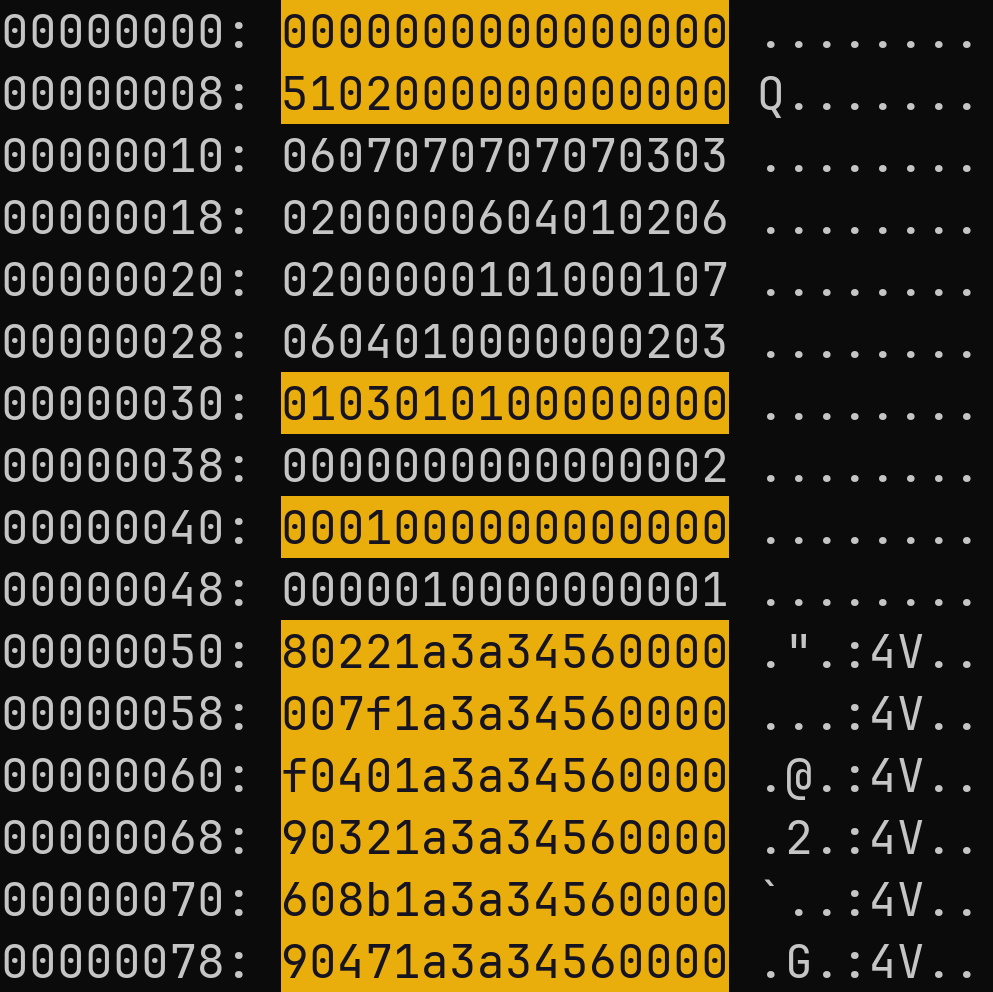
\includegraphics[width=16cm]{dataset/pointer_examples_1010-1644391327-heap_potential_pointer_highlight.png}

    We have information about the starting address of the heap using \lstinline[style=json]!"HEAP_START": "56343a198000"!. Considering that the example heap dump file contains $ 135169 $ bytes, this means that for this given heap dump file, the pointer addresses range from value $ 94782313037824_{10} $ and $ 94782313172993_{10} $. Note that the little-endian hexadecimal representation of the heap end address is \lstinline[language=c]!0x01901b3a3456! which is 12 character long, or 6 bytes long.

    Note that conversions here can get confusing, since potential pointer strings extracted from the heap dump file are given in little-endian hexadecimal format, but the heap start address from the JSON annotation file is given in big-endian hexadecimal format.

    \begin{minipage}{\dimexpr\linewidth-20pt}
        That way, we can refine the detection of potential pointers by only considering the bytes that are in the range of the heap. Potential pointers are highlighted with "<<<" in the following hex dump:

        \begin{lstlisting}[language=python, caption={Conversions function from hex strings to decimal $ int $ values}.]
        # conversion from hex to decimal
        def hex_str_to_int(hex_str: str) -> int:
            """
            Convert a normal (big-endian) hex string to an int.
            WARNING: HEAP_START in JSON is big-endian.
            """
            bytes_from_str = bytes.fromhex(hex_str)
            return int.from_bytes(
                bytes_from_str, byteorder='big', signed=False
            )
        
        def pointer_str_to_int(hex_str: str) -> int:
            """
            Convert a pointer hex string to an int.
            WARNING: Pointer hex strings are little-endian.
            """
            bytes_from_str = bytes.fromhex(hex_str)
            return int.from_bytes(
                bytes_from_str, byteorder='little', signed=False
            )
        \end{lstlisting}
    \end{minipage}

    Using the functions above, we can check which potential pointers are indeed within the heap dump range.

    \begin{minipage}{\dimexpr\linewidth-20pt}
        That way, we can refine the detection of potential pointers. In the following, pointers are highlighted with \lstinline[style=hexdump]!<<<! in the following hex dump:

        \begin{lstlisting}[style=hexdump, caption={8 bytes per line visualization of a Hex Dump from \textit{Training/basic/V\_7\_8\_P1/16/5070-1643978841-heap.raw}}]
            00000000: 0000000000000000 ........
            00000008: 5102000000000000 Q.......
            00000010: 0607070707070303 ........
            00000018: 0200000604010206 ........
            00000020: 0200000101000107 ........
            00000028: 0604010000000203 ........
            00000030: 0103010100000000 ........
            00000038: 0000000000000002 ........
            00000040: 0001000000000000 ........
            00000048: 0000010000000001 ........
            00000050: 80221a3a34560000 .".:4V.. <<<
            00000058: 007f1a3a34560000 ...:4V.. 
            00000060: f0401a3a34560000 .@.:4V.. <<<
            00000068: 90321a3a34560000 .2.:4V.. <<<
            00000070: 608b1a3a34560000 `..:4V.. <<<
            00000078: 90471a3a34560000 .G.:4V.. <<<
        \end{lstlisting}
    \end{minipage}

    \begin{minipage}{\dimexpr\linewidth-20pt}
        One last check we can do, is verify if the potential pointers are  8-bytes aligned. This can be done by checking if the last 3 bits of the potential address are 0, or using a modulo 8 operation. A simple python function can be used to check that:

        \begin{lstlisting}[language=python, caption={Python function to check if a potential pointer is 8-bytes aligned}]
            def is_pointer_aligned(pointer: int) -> bool:
                """
                Check if a pointer is 8-bytes aligned.
                """
                return pointer % 8 == 0
        \end{lstlisting}
    \end{minipage}

    Using this function on the potential pointers we have found so far, we can see that all of them are indeed 8-bytes aligned. This is a good sign for pointer detection, as we now have a range of tests that can be used to detect potential pointers from other potentially random values.

    Here is the pseudo-code for the pointer detection algorithm. This algorithm is presented for a full heap dump file:

    \begin{algorithm}
        \caption{Pointer Detection Algorithm}
        \begin{algorithmic}[1]
        \Procedure{PointerDetection}{$\text{heapDumpFile, HEAP\_START}$}
            \State $\text{heapStart} \gets \text{hex\_str\_to\_int}(HEAP\_START)$
            \State $\text{heapEnd} \gets \text{heapStart} + \text{FileSize}(\text{heapDumpFile})$
            \State $\text{position} \gets 0$
            \State $\text{potentialPointers} \gets []$
            \While{$\text{position} < \text{FileSize}(\text{heapDumpFile})$}
                \State $\text{block} \gets \text{Read8Bytes}(\text{heapDumpFile, position})$
                \If{$\text{block} \neq 0$}
                    \State $\text{pointer} \gets \text{pointer\_str\_to\_int}(\text{block})$
                    \If{$\text{heapStart} \leq \text{pointer} \leq \text{heapEnd}$}
                        \If{$\text{is\_pointer\_aligned}(\text{pointer})$}
                            \State $\text{Append}(\text{pointer}, \text{potentialPointers})$
                        \EndIf
                    \EndIf
                \EndIf
                \State $\text{position} \gets \text{position} + 8$
            \EndWhile
            \State \Return $\text{potentialPointers}$
        \EndProcedure
        \end{algorithmic}
    \end{algorithm}

    This pseudo-code outlines the steps for detecting potential pointers in the heap dump file. It starts by reading the heap dump file 8 bytes at a time. For each 8-byte block, it checks if the block is non-zero and within the heap range. If so, it checks if the potential pointer is 8-bytes aligned using the \texttt{is\_pointer\_aligned} function we described before. If all conditions are met, the potential pointer is added to the list of potential pointers. The algorithm returns this list at the end.
    
    \subsubsection{Detecting potential keys}
    % speak about SmartKex22 brute force approach
    % describe the algorithm to detect potential keys

    Encryption key prediction is the main focus of the present thesis. As such, we will now focus on how to detect potential keys in heap dump files. The paper \citetitle{SmartKex22} introduces 2 algorithms for key detection. The first one is a brute force approach that consists in trying all the possible keys in the heap dump file. The second one is a more sophisticated approach that uses a set of rules to detect potential keys.
    
    The first brute-force algorithm is given by:

    \begin{algorithm}[H]
    \caption{SSH keys brute-force algorithm from \citetitle{SmartKex22} \cite{SmartKex22}}
    \begin{algorithmic}[1]
    \Procedure{FindIVAndKey}{$\text{netPacket}, \text{heapDump}$}
        \State $\text{ivLen} \gets 16$ \Comment{Based on the encryption method}
        \State $\text{keyLen} \gets 24$ \Comment{Based on the encryption method}
        \State $i \gets \text{sizeof(cleanHeapDump)}$
        \State $r \gets 0$
        \While{$r < i$}
            \State $\text{pIV} \gets \text{heapDump}[r : r + \text{ivLen}]$
            \State $x \gets 0$
            \While{$x < i$}
                \State $\text{pKey} \gets \text{heapDump}[x : x + \text{keyLen}]$
                \State $f \gets \text{decrypt}(\text{netPacket}, \text{pIV}, \text{pKey})$
                \If{$f$ is TRUE}
                    \State \textbf{return} $\text{pIV}, \text{pKey}$
                \EndIf
                \State $x \gets x + 8$ \Comment{The IV is 8-bytes aligned}
            \EndWhile
            \State $r \gets x + 8$ \Comment{The key is 8-bytes aligned}
        \EndWhile
    \EndProcedure
    \end{algorithmic}
    \end{algorithm}
    
    Algorithm~1 outlines the brute-force approach for finding the Initialization Vector (IV) and the key. Initially, the lengths \(\text{ivLen}\) and \(\text{keyLen}\) are set based on the encryption method used for the heap. The algorithm then takes the first \(\text{ivLen}\) bytes from the heap dump to serve as the potential IV (\(pIV\)). Subsequently, \(\text{keyLen}\) bytes are extracted from the heap dump, starting from the first byte, to act as the potential key (\(pKey\)). The algorithm iterates through this potential key until it reaches the end of the heap dump. If decryption of the network packet is unsuccessful, the process is repeated by reading the next potential IV and the subsequent potential key \cite{SmartKex22}. 

    This algorithm is fairly straightforward, and can be implemented in a few lines of code. However, it is also very inefficient, as it tries all the possible keys in the heap dump file. It also needs some encrypted network packets to be able to test the keys, which are not included in the dataset. As such, we will not implement this algorithm.
    
    This is why the authors of the paper have also developed a more sophisticated algorithm that uses a set of rules to detect potential keys.

    No pseudo-code is given for the second algorithm, but the paper \citetitle{SmartKex22} gives a description of the algorithm. It rely on the high-entropy assumption of encryption keys. The algorithm is inspired by image processing techniques, and can be described as follows:

    \begin{algorithm}
        \caption{Image-processing inspired Preprocessing Algorithm, as described in \citetitle{SmartKex22} \cite{SmartKex22}}
        \begin{algorithmic}[1]
        \Procedure{Preprocessing}{$\text{heapData}$}
            \State \textbf{Reshape} $\text{heapData}$ into $N \times 8$ matrix $X$
            \For{$i = 0$ to $N-1$}
                \For{$j = 0$ to $7$}
                    \State $Y[i][j] = |X[i][j] - X[i][j+1]| \& |X[i][j] - X[i+1][j]|$
                    \State $Z[i] = \text{count}(Y[i][k] == 0) \geq 4$
                    \If{$i < N-1$}
                        \State $R[i] = Z[i] \& Z[i+1]$
                    \EndIf
                \EndFor
            \EndFor
            \State \textbf{Extract} 128-byte slices from $R$ for training
        \EndProcedure
        \end{algorithmic}
    \end{algorithm}
    
    This Preprocessing Algorithm serves as a crucial step in adapting the heap data for machine learning models. The algorithm begins by reshaping the raw heap data into an \(N \times 8\) matrix \(X\), since keys are 8-bytes aligned \cite{SmartKex22}. Here, \(N \times 8\) is the size of the original heap data in bytes. It then calculates the discrete differences of the bytes in both vertical and horizontal directions, storing the results in matrix \(Y\). The algorithm employs a logical AND operation on these differences to identify high-entropy regions, which are likely candidates for encryption keys. Each 8-byte row in \(Y\) is examined for randomness, and if at least half of its bytes differ from adjacent bytes, it is marked as a potential part of an encryption key. The algorithm then filters out isolated rows that are unlikely to be part of an encryption key, resulting in an array \(R\). Finally, 128-byte slices are extracted from \(R\) for training the machine learning model. This preprocessing step not only adapts the data for machine learning but also narrows down the search space for potential encryption keys, thereby enhancing the efficiency of the subsequent steps. 

    However, this algorithm is not as efficient as it could be. It rely on using a kind of sliding window, which is not easily parallelizable. Also, the entropy-inspired computation is not as straightforward as it could be. That why we propose a new algorithm that is more efficient and more easily parallelizable.

    In order to perform some \acrshort{ml} techniques, and because the keys we are looking for can have a range of possible lengths (16, 24, 32, or 64 bytes), we shift the focus from detecting the full key, to just be able to predict the address of the key. That way, we can deal with keys of different sizes, and we can also use the same algorithm to detect the IV. This is why we will focus on detecting potential keys addresses, and not the full keys.

    We thus introduce a new algoritm for narrowing the search space for potential keys. This algorithm is inspired by the paper \citetitle{SmartKex22}, but is more efficient and more easily parallelizable, as it focuses on producing pairs of blocks of 8 bytes with high entropy. It uses directly the Shannon entropy formula, with each entropy computation being independent from the others.

    \begin{algorithm}
        \caption{Entropy Based Detection of Potential Key blocks}
        \begin{algorithmic}[1]
        \Procedure{EntropyDetection}{$\text{heapData}$}
            \State \textbf{Pad} $\text{heapData}$ with 0s to be 8-bytes aligned
            \State \textbf{Reshape} $\text{heapData}$ into $N \times 8$ matrix $X$
            \For{$i = 0$ to $N-1$,}
                \State $entropy[i] = \text{ShannonEntropy}(X[i])$ \Comment{Independents, compute in parallel.}
            \EndFor
            \State \textbf{Add} $entropy$ 2 by 2 pairs into $entropy\_pairs$ \Comment{Keep block indexes in resulting tuples.}
            \State \textbf{Sort} $entropy\_pairs$ by entropy as $sorted\_pairs$
            \State \Return $\text{SortedPairs}(\text{sorted\_pairs})$
        \EndProcedure
        \end{algorithmic}
    \end{algorithm}

    The \textit{Entropy Based Detection of Potential Key blocks} algorithm takes a raw heap dump, represented by the variable \texttt{heapData}, as input. The data is first padded with zeros to align it to 8-byte blocks and then reshaped into an $N \times 8$ matrix $X$. The Shannon entropy is computed for each 8-byte block in parallel, resulting in an array \texttt{entropy}. Subsequently, the entropy values of adjacent blocks are summed to form pairs, which are stored in \texttt{entropy\_pairs} along with their block indexes. These pairs are then sorted by their entropy sums to produce \texttt{sorted\_pairs}. The idea of using pairs of blocks instead of a single block or more that two blocks is related to the minimim key size, which is 16 bytes. This means that we need at least 2 blocks to be able to detect a potential key. The algorithm returns sorted pairs, so that we can easily extract the ones with the highest entropy sums. Given the index of a block, its actual memory address can be recomputed using the \texttt{HEAP\_START} address available in annotations.
    
    Using this algorithm, let's continue to explore our example heap dump file from \autoref{lst:hexdump-8bytes}. We will use the following python function to compute the Shannon entropy of a given block of 8 bytes:

    \begin{minipage}{\dimexpr\linewidth-20pt}
    \begin{lstlisting}[language=python, caption={Python function to compute the Shannon entropy of a given block of 8 bytes}]
        def get_entropy(data: bytes):
            """
            Computes the entropy of a byte array, using Shannon's formula.
            """

            if len(data) == 0:
                return 0.0
            
            # Count the occurrences of each byte value
            _, counts = np.unique(data, return_counts=True)
            
            # Calculate the probabilities
            prob = counts / len(data)
            
            # Calculate the entropy using Shannon's formula
            entropy = -np.sum(prob * np.log2(prob))
            
            return entropy
    \end{lstlisting}
    \end{minipage}

    This function used np array function for efficient computation. We can now use this function to compute the entropy of each block of 8 bytes in the heap dump file. We can then sort the pair of blocks by their entropy, and keep the ones with the highest entropy.
    
    When applied to the file \textit{Training/basic/V\_7\_8\_P1/16/5070-1643978841-heap.raw}, the algorithm produced $ 16896 $ entropy pairs, with $ 631 $ pairs having the maximum entropy sum. Another test using the index to address conversion and the JSON annotation file also indicate that all of the 6 key addresses are within the $ 631 $ pairs with the highest entropy sum.
    
    This allows to reduce significantly the search space for potential keys, to already less that 4\% of the original heap dump file, which is significantly better that the 30\% reduction obtained by the preprocessing algorithm described in the paper SmartKex \cite{SmartKex22}, but less that the 2\% reduction obtained by the \acrshort{ml}-based processing algorithm described in the paper \cite{SmartKex22}. However the same paper indicated that it was tested only for Key A and Key C, whereas this algorithm is tested for all the keys. Keep in mind that this is just an example for a single random file in the dataset, as a way to introduce the subject. In-depth experiments will be done in the dedicated chapter on \acrlong{ml}.

    Indeed, it is important to mention that we can rely on the JSON annotation files for providing labelling for key address prediction. Using this, we do not need to decrypt the network packets to be able to train our \acrshort{ml} models. This is a huge advantage, and is also required since we don't have the encrypted network packets in the dataset. Since we don't have those, and since the keys are already given, that is why we will focus on key address prediction, and not on key prediction.

    \subsubsection{Detecting potential data structures}
    Since the dataset contain whole heap dump file, we can also try to detect potential data structures in those heap dumps. This can be done by looking for patterns in the heap dump file, in a similar fashion as we have done for potential pointers.
    
    Since OpenSSH is written in C, we can expect to find some C data structures in the heap dump files. C uses the \lstinline[language=c]|malloc| function to allocate memory. This function is used to allocate memory for a given data structure. This function takes as input the size of the data structure to allocate, and returns a pointer to the allocated memory. Looking at the code \footnote{The dataset has been produced on a \texttt{x86\_64} architecture, so as an example code, we have looked at uClibc for a \lstinline[language=c]|malloc| implementation: \url{https://git.busybox.net/uClibc/tree/libc/stdlib/malloc/malloc.c} } for \lstinline[language=c]|malloc|, we can see the following:
    
    \begin{minipage}{\dimexpr\linewidth-20pt}
        \begin{lstlisting}[language=c, caption={Malloc implementation for uclibc}]
        /* Include extra space to record the size of the allocated block.  */
        size += MALLOC_HEADER_SIZE;
        \end{lstlisting}
    \end{minipage}
    
    A \lstinline[language=c]|malloc| call is expected to allocate a memory block of the size of the data structure, plus 8 bytes (). This is because the \lstinline[language=c]|malloc| function also stores some metadata about the allocated memory block. This metadata is stored in the bytes that are allocated in addition to the data structure size. This is why we can expect to find some 8-bytes aligned blocks in the heap dump file, that are not pointers, but that are the result of a \lstinline[language=c]|malloc| call. Detecting and using those \textit{malloc headers} is how we will also try to detect potential data structures in the heap dump file.

    We don't know which implementation of \lstinline[language=c]|malloc| has been used for the OpenSSH programs used to generate the dataset. However, we can expect it to be similar to the one used in uclibc, a lightweight C library that is often used in embedded systems. 

    In Linux on a \texttt{x86\_64} architecture, the malloc function typically uses a block (chunk) header to store metadata about each allocated block. This header is placed immediately before the block of memory returned to the user. The exact layout can vary depending on the implementation of the C library (e.g., glibc, musl), but generally, it contains the following:

    \begin{itemize}
        \item \textbf{Size of the Block}: The size of the allocated block, usually in bytes. This size often includes the size of the header itself and may be aligned to a multiple of 8 or 16 bytes.
        \item \textbf{Flags}: Various flags that indicate the status of the block, such as whether it is free or allocated, or whether the previous block is free or allocated. These flags are often stored in the least significant bits of the size field, taking advantage of the fact that the size is usually aligned, leaving the least significant bits zeroed.
    \end{itemize}
    
    Since the malloc header respects the endianness of the system, we can expect to find the malloc header in little-endian format in the heap dump file. Using vim on \textit{Training/basic/V\_7\_8\_P1/16/5070-1643978841-heap.raw}, we can use the following command to find some potential malloc headers:

    \begin{lstlisting}[language=bash, caption={Vim command to find potential malloc headers}]
        :/[0-9a-f]\{4}0\{12}
    \end{lstlisting}
    
    This gives something like the following:

    \begin{figure}[H]
        \centering
        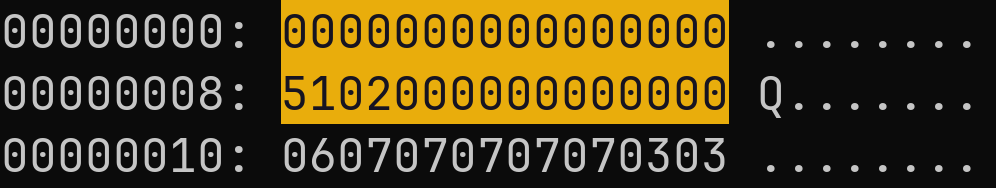
\includegraphics[width=16cm]{dataset/structure_examples_1010-1644391327-heap_potential_malloc_header_highlight_heap_start.png}
        \caption{Attempt at malloc header detection in \textit{Training/basic/V\_7\_8\_P1/16/5070-1643978841-heap.raw}, at heap start.}
    \end{figure}

    Indeed, after a first zero block of 8 bytes, we expect a first data structure to be allocated at the start of the heap. Here this data structure is of size $ 5102000000000000_{16LE} $ (little-endian hex format) or $ 593_{10} $ bytes. The fact that it is an odd number is due to the \acrshort{lsb} being set to 1, to indicate that the block is allocated (flag). This means that the real size of the structure is actually $ 593_{10} - 1_{10} = 592_{10} $. This value is 8-byte aligned.

    Since we know that the allocator allocates chunks after chunks, we can expect the next chunk to be allocated at the address $ 5102000000000000_{16LE} + 592_{10} + 8_{10} = 5882193a34560000_{16LE} =  $. Note that we need to add 8 to the size to account for the malloc header block.
    
    In vim, since the address start at 0, we have to look at $ 592_{10} + 8_{10} = 258_{16} $. Let's have a look there:

    \begin{figure}[H]
        \centering
        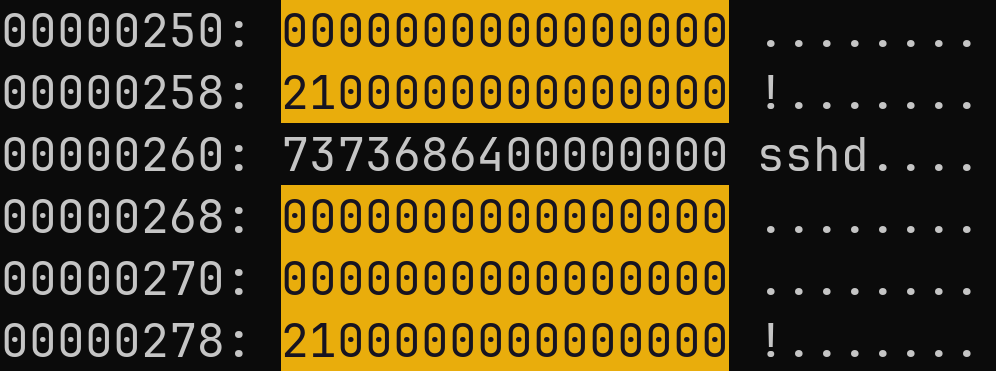
\includegraphics[width=16cm]{dataset/structure_examples_1010-1644391327-heap_potential_malloc_header_highlight_0x250.png}
        \caption{Attempt at malloc header detection in \textit{Training/basic/V\_7\_8\_P1/16/5070-1643978841-heap.raw}, at index $ 592_{10} = 250_{16} $.}
    \end{figure}

    There, we can see a zero block, followed by what we can expect to be another malloc header at address $ 258_{16} $. By doing the same process, we can thus propose an algorithm to detect the malloc headers, and thus the structures in the heap dump file.

    \begin{algorithm}[H]
        \caption{Malloc Header Detection Algorithm}
        \begin{algorithmic}[1]
        \Procedure{MallocHeaderDetection}{$\text{heapDumpFile}$}
            \State $\text{position} \gets 0$
            \While{$\text{position} < \text{FileSize}(\text{heapDumpFile})$}
                \State $\text{block} \gets \text{Read8Bytes}(\text{heapDumpFile, position})$
                \If{$\text{block} \neq 0$}
                    \State $\text{size} \gets \text{ConvertToSize}(\text{block}) - 1$ \Comment{$-1$ due to the flag}
                    \State \textbf{Assert} $ \text{size} \mod 8 = 0$ \Comment{Check if the size is 8-bytes aligned}
                    \State $\text{position} \gets \text{position} + 8 + \text{size}$ \Comment{Leap over data structure. + 8 for the header.}
                \Else
                    \State $\text{position} \gets \text{position} + 8$
                \EndIf
            \EndWhile
        \EndProcedure
        \end{algorithmic}
    \end{algorithm}

    The idea behing the malloc header detection algorithm is simple. We start at the beginning of the heap dump file, and we look for the first non-zero block. We then assume that the next block is a malloc header. We convert it to a size, and then leap over the data structure and the header. The process is repeated until reaching the end of the heap dump file.

    \section{Hardware and software architecture}
    Throughtout this thesis, we have used a variety of hardware and software architectures. 
    
    \subsection{Hardware development and testing environment}
    In this section, as a reference for the reader, we will describe shortly the hardware development environment. All environments are running some Linux \texttt{x86\_64} distribution.

    At the start of the project, around the end of 2022, the project started on a old laptop \textit{HP EliteBook Folio 1040 G2}, running \texttt{Ubuntu 22.04 LTS (Jammy Jellyfish)} with the following specifications:

    \begin{itemize}
        \item \textbf{CPU:} 5th Generation Intel Core i7-5600U 2.6 GHz (max turbo frequency 3.2-GHz), 4 MB L3 Cache, 15W
        \item \textbf{GPU:} Intel HD Graphics 5500
        \item \textbf{RAM:} 8GB DDR3L SDRAM (1600 MHz, 1.3v)
    \end{itemize}

    This device was used for the first experiments, and for the development of the first programs. However, it was not powerful enough to run the experiments on the whole dataset, and especially working on \acrshort{ml} part. As such, we have moved to a more powerful machine, a \textit{TUXEDO InfinityBook Pro 16 - Gen7} with the following specifications:

    \begin{itemize}
        \item \textbf{CPU:} 12th Gen Intel i7-12700H (20) @ 4.600GHz
        \item \textbf{GPU:} NVIDIA Geforce RTX 3070 Ti Laptop GPU
        \item \textbf{RAM:} 64GB DDR5 4800MHz Samsung
    \end{itemize}

    For the Operating System, we have switched from \texttt{Fedora 37} to \texttt{NixOS 23 (Tapir)}. This change was motivated by the fact that \texttt{NixOS} is a Linux distribution that uses a purely functional package management system \cite{NixOS08}. This means that the operating system is built by the Nix package manager, using a declarative configuration language. This allows to have a reproducible development environment, and to easily switch between different development environments. This has proved to be very useful in many areas like work environment isolation, on work collaboration with Clément Lahoche, and for software deployment to the server.
    
    Unfortunatly, the \textit{TUXEDO InfinityBook Pro 16 - Gen7} laptop was not powerful enough to run the experiments on the whole dataset. Running the python script would have taken more than a week for some simple \acrshort{ml} experiments to run on the whole dataset, and even reprogrammed and better optimized programs in Rust that we have tested would take more that 10 hours to process the dataset. Small bash and python scripts have been run on this laptop, but all the main experiments have been run on the server.
    
    In that context, we were provided a development server towards the end of the thesis, around august 2023. This server is a \textit{AS-4124GS-TNR} with the following specifications:

    \begin{itemize}
        \item \textbf{CPU:} 2x AMD EPYC 7662 (256) @ 2.000GHz
        \item \textbf{GPU:} NVIDIA Geforce RTX 3090 Ti
        \item \textbf{RAM:} 512GB DDR4 3200MHz
    \end{itemize}

    This server is running \texttt{Ubuntu 20.04.6 LTS} and is used to run the \acrshort{ml} experiments on the dataset, as it is much more powerful than the laptop. This server has be provided by the Department of Computer Science of Universität Passau, and especially the Chair of Data Science of Prof. Dr. Michael Granitzer. We would like to thank them for their support.

    \subsection{Software, languages and tools}
    In Computer Sciences, it does't take long to realize that testing hypotheses, diving deeper in problems and finding solutions to them is a very iterative process that requires a lot of experimentation. As such, the development of scripts and programs has been a substantial part of this thesis, from the very beginning to the very end. In this process, we have used a variety of tools and programming languages, such as Rust, Python, Bash, or Nix just to name the programming language used.

    In this section, as a reference for the reader, we will describe the software architectures, languages and tools that have been used throughout this thesis.

    Throughtout the project, we have come to use a range of programming languages. Initial tests have been done using shell and bash command and simple scripts. However, as the project grew, we quickly moved to more powerful programming languages. 

    Python version 3.11 has been the main language for high level data science and \acrshort{ml} development. This new version of python features many improvements over the previous version, and especially in terms of performance. Better error messages, exception groups, improved support for f-strings, support for TOML configuration files, variadic generics, improved support for asyncio, and new modules for working with cryptography and machine learning are just some of the new features of this new version of python. While relatively new, this is why we have decided to use this version of python for the development of the \acrshort{ml} part of the project.

    Although Python is a popular and powerful language, it is not the most efficient language. As such, we have used Rust for some parts of the project, especially when no high level library is needed and when performances are critical to be able to parse efficiently the dataset. Rust is a systems programming language that runs blazingly fast, prevents segfaults, and guarantees thread safety. It is a very powerful language, and is especially useful for low-level programming. We have used it for the development of the algorithms that are used to extract the data from the dataset.

    \subsubsection{Packaging and deployment}
    We made an extensive use of git repositories for version control, with GitHub as a main platform for hosting the repositories. An ever growing number of script and programs have been developed for this thesis. As such, we have needed a way to easily deploy those programs on different machines.

    Rust comes with a handful of tools for managing packages and dependencies. Cargo is Rust's build system and package manager. Cargo downloads your Rust project's dependencies, compiles your project, makes executables, and runs the tests. It is a powerful tool that allows to easily manage Rust projects. However, it is not the best tool for deploying programs on different machines. 

    On Python's side of things, things are a bit more complicated. For a long time, we have relied on virtual environments using the \texttt{conda} package manager. However, it is heavy to use, and it doesn't allow to easily export an environment from one linux distribution to the other. This was especially a problem when development was done on a Fedora system but the server was running Ubuntu. 

    An example is the library \texttt{pygraphviz}. This library relies on third parties system libraries, that have different names depending on the linux distribution:
    
    \begin{itemize}
        \item \textbf{Ubuntu:} \lstinline[language=bash]|sudo apt-get install graphviz graphviz-dev| is needed before a correct install of the Python \texttt{pygraphviz} library. 
        \item \textbf{Fedora:} \lstinline[language=bash]|sudo dnf install graphviz graphviz-devel| is needed before installing \texttt{pygraphviz}
    \end{itemize}

    Although it can be seen as a minor issue, this is just one example among dozens of libraries. This is real problem with \texttt{conda}. This is why we have decided to use Nix for managing python packages and dependencies. Nix is a purely functional package manager \cite{NixOriginalThesis06}. It allows to easily manage packages and dependencies, and to easily deploy programs on different machines as it guarantees reproducible builds. It is also very useful for development, as it allows to easily create isolated environments for development. This is why we have used Nix for managing the python packages and dependencies. Gradually, Nix has become a superset of other package managers like pip, conda, or cargo. 
    
    Any Nix project comes with either a \textit{shell.nix} or a more modern \textit{flake.nix}. Those files are used to describe the project, and to list all necessary dependencies. Since we are developping on NixOS, the integration of Nix with the operating system is very good, and can be easily setup.
    
    Nix is however really straightforward to install on any other distribution through the use of a single script available online. It can be install in as little as one command.


%\section{Programs development}
% describe the programs developped for the Masterarbeit
% * mem2graph

% In Computer Sciences, it does't take long to realize that testing hypotheses, diving deeper in problems and finding solutions to them is a very iterative process that requires a lot of experimentation. As such, the development of scripts and programs has been a substantial part of this thesis, from the very beginning to the very end. In this process, we have used a variety of tools and programming languages, such as Rust, Python, Bash, or Nix just to name the programming language used. In this section, we will do a general overview of the programs we have developed for this thesis. More details about the programs will be discussed further in their respective chapters.


% In this section, we will describe the programs we have developed for this thesis. We will first describe the program we have developed to explore the dataset. Then, we will describe the program we have developed to extract the data from the dataset. Finally, we will describe the program we have developed to analyze the data.

\section{Converting memory dumps to graphs}\label{chap:mem_2_graph}
Now that we have a decent understanding of the dataset as well as the low level memory dump format, we can start to think about how to convert the memory dumps into graphs. As a recall, we want to be able to convert a memory dump into a graph representation that can be used for machine learning, since we want to be able to create a memory modelization as a basis for efficient embedding and feature engineering later. This is inherently due to the imbalanceness of the dataset, as we want to add more information to each memory block that just its raw bytes. The goal is to have a graph representation of the memory dump that can be used for efficient machine learning.

This section will be dedicated to describe the methods developped around this problem. We will first discuss the design of the graph representation, then we will discuss the implementation of the graph construction process. Finally, we will discuss the semantic embedding of the graph, which is the process of adding more information to the graph.

\subsection{Initial work from Python to Rust}

\subsubsection{First steps}
    Initially, we have been working and manipulating the code provided by SmartKex\footnote{SmartKex GitHub repository: \url{https://github.com/smartvmi/Smart-and-Naive-SSH-Key-Extraction}} for key detection. Our first explorations of the dataset quickly gave birth to some Jupyter Notebooks, which were used to explore the dataset and to understand the code, like \texttt{search\_in\_heap\_mem.ipynb}. Rapidly, we decided to rebuild a complete Python 3.11 version of the code. This was done for several reasons:

    \begin{itemize}
        \item The original code has no type hinting, which makes it hard to read and understand.
        \item We wanted to explore the dataset and learn by doing.
        \item The original code was not designed to be used as a library, but rather as a standalone script.
        \item The original code was just a few hundred lines of code and was not designed to be easily extensible, nor to be able to handle a large number of memory dumps.
    \end{itemize}

    We decided to build a memory graph representation at that moment because we wanted to be able to add more information to the memory blocks than just their raw bytes. This new program was called \texttt{ssh\_key\_discover}, and relied on a number of Python libraries to work, like \texttt{graphviz}. This was a all-in-one library, composed of 2 sections, \texttt{mem\_graph} and \texttt{ml\_discovery}. The first one is dedicated to building the memory graph, while the second one is dedicated to the data science and machine learning part.

    This initial program was already capable of handling several data processing pipelines, including machine learning pipelines with models like Random Forest, a grid search for hyperparameter optimization, and a cross validation pipeline, several balancing strategies and of course, a memory graph representation and semantic embedding. As an early development version, this program was not optimized for performance, and just loading a given heap dump file and its annotation, and then building the memory graph representation, could take from 30 seconds to a minute (on the TUXEDO machine), depending on the size of the heap dump file. As we are dealing with more that $ 10^{6} $ files, a rapid estimation of the time needed just for the semantic embedding of the memory graph representation was above a month. In this regard, this initial program was just used on a bunch of files as a way to develop the semantic embedding model, algorithm and start working on feature engineering and machine learning.
    
    This optimization issue was clearly not acceptable, and we decided to rewrite the graph part in Rust, which is a compiled language, and thus, several order of magnitude faster than Python. This was also a good opportunity to learn Rust, which is a language that is gaining more and more popularity, especially in the security community. This new program was called \texttt{mem2graph}. Switching from Rust to Python and doing a proper use of multithreading allowed us to reduce the time needed to build the memory graph representation from 30 seconds to less than 1 second. In out case, and comparing using only the TUXEDO laptop, this represent an estimated minimum of a 130x speedup. But this is even much better on the server, where the multithreading can really be leverage. This was a huge improvement, and allowed us to build the memory graph representation for the whole dataset in a just a few hours.

\subsection{Memory Graph Representation}
Now, let's describe the memory graph representation. The goal is to be able to represent a memory dump as a graph. This modelization makes sense since the heap dump can be considered as having data structures as nodes, being connected by pointers acting as arrows. This is a very natural way to represent a memory dump. However in our cases, and since the goal is to make predictions on raw bytes, we will not use the data structures as nodes, but rather the memory blocks directly. This is because we want to be able to make predictions on raw bytes, and not on data structures. 

% introduce the type of the graph, the nodes and edge
The main idea behind the following memory graph representation is to be able to represent the whole content of a heap dump file as a directed graph that contains the address as well as the byte block of every element. This last point is especially important since we want to be able to make predictions on raw bytes, and not on data structures. This is why we will not use the data structures as nodes, but rather the memory blocks directly. 

In the 

\subsection{Graph Construction}
% graph construction algorithm
% graph annotation algorithm

\subsection{Exporting the Graph}
% the DOT format


\begin{minipage}{\dimexpr\linewidth-20pt}
    Here are the constants define for memory format conversion in the Rust code:

   %\begin{lstlisting}[language=json, , label={lst:json}]
   \begin{lstlisting}[style=rust, caption={Rust memory format constants in \textit{mem2graph}}]
    pub const BLOCK_BYTE_SIZE: usize = 8; // 64-bit, ex: C0 03 7B 09 2A 56 00 00
    pub const PTR_ENDIANNESS: Endianness = Endianness::Little;
    pub const MALLOC_HEADER_ENDIANNESS: Endianness = Endianness::Little;
   \end{lstlisting}
\end{minipage}

\subsection{Semantic Embedding}\label{sec:mem_2_graph:semantic_embedding}
% semantic embedding algorithm
% the CSV embedding format



%\section{Packaging and deployment with Nix}
\section{Feature engineering}
% describe the feature engineering process

\section{ML for key prediction}
% this is composed of the classical ML pipelines and of the GCN pipelines

The chapter has been an overview of the dataset, development environment, and tools used for this thesis. In the next chapter, we will dive deeper into the graph memory representation and associated algorithms and programs.

